\section{应用领域}
\subsection{机器人与具身人工智能}
在机器人系统中，世界模型承担多种互补角色：作为预测模拟器用于策略评估与规划；作为表征学习器，从大规模观测中捕捉任务相关动力学；并且越来越多地作为数据引擎，生成用于下游策略训练的合成经验。这些能力在具身场景中尤其重要，因为采集真实交互数据代价高昂，智能体又必须跨多样任务、环境、物体和机器人本体进行泛化。

生成建模的近期进展，大幅拓展了机器人世界模型的范围与有效性。受大规模视频生成模型成功的启发\citep{rombach2022high}，越来越多的工作超越紧凑潜在状态预测，转向基于视频的世界建模，显式生成未来视觉观测并用于决策。这些模型利用大规模视频数据集中丰富的时空知识，已用于机器人操作、导航、策略评估、强化学习和合成数据生成。在这一趋势之上，近期世界行动模型（WAM）在统一生成框架中联合建模未来观测与机器人行动\citep{hu2024video,ye2026dreamzero}。WAM不将规划与控制视为独立阶段，而是学习未来世界状态与行动的联合分布，使行动预测直接受益于所学环境动力学。代表工作表明，将世界建模目标与行动预测结合，可以提高样本效率、鲁棒性、跨本体迁移，以及对新任务和新环境的泛化能力。更重要的是，WAM继承互联网规模视频预训练的视觉与物理先验，为可扩展具身智能指明了一条有前景的道路：生成式世界建模的进步可以直接转化为机器人能力的提升。因此，世界模型日益被视为面向未来具身智能体、整合感知、预测、模拟和行动生成的统一框架，而不只是规划模块。

除WAM所体现的统一“感知—预测—行动”表述外，世界模型对机器人系统的功能贡献，还可以沿三个互补维度更明确地区分。这些维度的区别，在于具身智能体流程在\emph{何时}、以多少计算预算使用预测未来。

\paragraph{数据引擎。}
在离线模式中，可以反复查询所学世界模型，并与实时控制解耦，合成大量在视觉与物理上合理的交互数据，以补充或替代昂贵的遥操作演示。近期具有组合性、考虑本体差异的世界模型具体展示了这一角色：RoboDreamer将语言条件视频生成分解为可复用基元，以合成未见物体与行动组合的计划\citep{zhou2024robodreamer}；UniSim则将异构图像、机器人和导航数据组织为通用交互模拟器，使高层与低层策略都能先完全在想象中训练，再零样本迁移到真实世界\citep{yang2024unisim}。

\paragraph{环境模拟器。}
这类用法不是生成训练数据，而是在评估时查询模型，通过推演预测后果，为候选策略、行动序列或超参数评分、排序，从而降低部署前物理试错的成本与风险。这一思想可追溯至Ha与Schmidhuber最初的世界模型：策略完全在学习得到的“梦境”环境中训练、评估，再迁移回真实环境\citep{ha2018worldmodels}。在机器人与驾驶场景中，MILE联合学习世界模型和驾驶策略，使复杂机动先完全通过想象规划和评估，再在CARLA模拟器中检验\citep{hu2022mile}。ReSim则针对只用安全专家数据训练的驾驶世界模型，遇到危险或非专家行为便容易失效的问题，明确关注这种计算机内评估的可靠性\citep{yang2025resim}。一条互补的非生成式路线，通过高保真渲染模拟而非学习动力学追求相同功能目标：SIMPLER表明，精心构建的模拟环境可以作为真实操作策略评估的可扩展、可复现替代，其结果与真实机器人表现高度相关，同时避免物理测试的成本与复现困难\citep{li2024simpler}。

\paragraph{行动规划器。}
第三种角色将世界模型直接嵌入控制循环，以低延迟在线查询，在候选行动条件下推断合理的近期状态，支持物理部署实时约束下的滚动时域规划（receding-horizon planning）或基于想象的规划。DayDreamer早期展示了这种模式：无需外部模拟器，直接在真实四足机器人和机械臂上学习潜在动力学并行动\citep{wu2022daydreamer}。

\paragraph{机器人本体世界模型。}
上述角色都涉及以智能体行动为条件，对\emph{外部环境}动力学建模。另一条正交且相对研究不足的路线，针对智能体自身的\emph{身体}：它不问给定行动后世界会发生什么，而是问，为达到目标或满足控制要求，智能体自身身体能够产生哪些行为。近期提出的行为基础模型（Behavior Foundation Model，BFM）在人形机器人全身控制中体现了这一方向\citep{zeng2025bfm}。现有全身控制框架仍大多针对特定任务，依赖繁重的人工奖励设计；由此出发，BFM在大规模行为数据上预训练，将掩码在线蒸馏框架与条件变分自编码器结合，对可行人形行为的广泛、可复用分布建模，随后可在不同控制模式下引导，或快速适应新行为，无需从头重训。世界模型编码外部场景如何演化的生成先验，而BFM及相关行为基础模型，编码受身体形态约束的自身技能流形上的生成先验，更像内部身体图式（body schema），而非外部场景模型。

我们认为，这两类生成先验——关于世界的先验和关于身体的先验——互补而非竞争。对于既要预期环境后果，又要知道自身身体能做什么的通用具身智能体，整合二者是一条有前景、且大体仍待探索的方向。

\textbf{驾驶模拟器。}
一类驾驶世界模型已经出现，明确将驾驶场景的演化，表述为给定过去观测与自车行动时，对未来感官观测进行条件生成的问题。GAIA-1以视频、文本与行动输入为联合条件，生成逼真的未来驾驶视频，表明大规模视频—行动预训练赋予模型对交通惯例和智能体动力学的隐式理解，使其还可充当生成训练与验证数据的神经模拟器\citep{hu2023gaia1}。DriveDreamer完全从真实驾驶场景构建世界模型，利用扩散模型表示结构化交通约束，同时支持可控视频生成和未来驾驶行动预测\citep{wang2023drivedreamer}。Vista进一步将这一范式扩展至具有泛化能力、高保真度的预测，支持跨异构行动表征的多样控制，明确针对早期驾驶世界模型对未见环境泛化有限、容易丢失安全关键细节的问题\citep{gao2024vista}。在这些系统中，时间维度不是附带因素，而是构成性要素：自动驾驶需要同时处理短时域反应式预测，例如即刻避撞，以及用于路线级决策的较长时域轨迹预测。驾驶世界模型通过在所学潜在空间或像素空间中自回归推演，将二者的计算摊入模型。从这一角度看，场景预测与轨迹预测不是独立子模块，而是同一底层预测基础的两个时间耦合实现，在显式生成、时间延展的框架内，重新体现了UniAD最初强调的联合感知—规划目标。

\subsection{科学发现}
\begin{figure}[t]
    \centering
    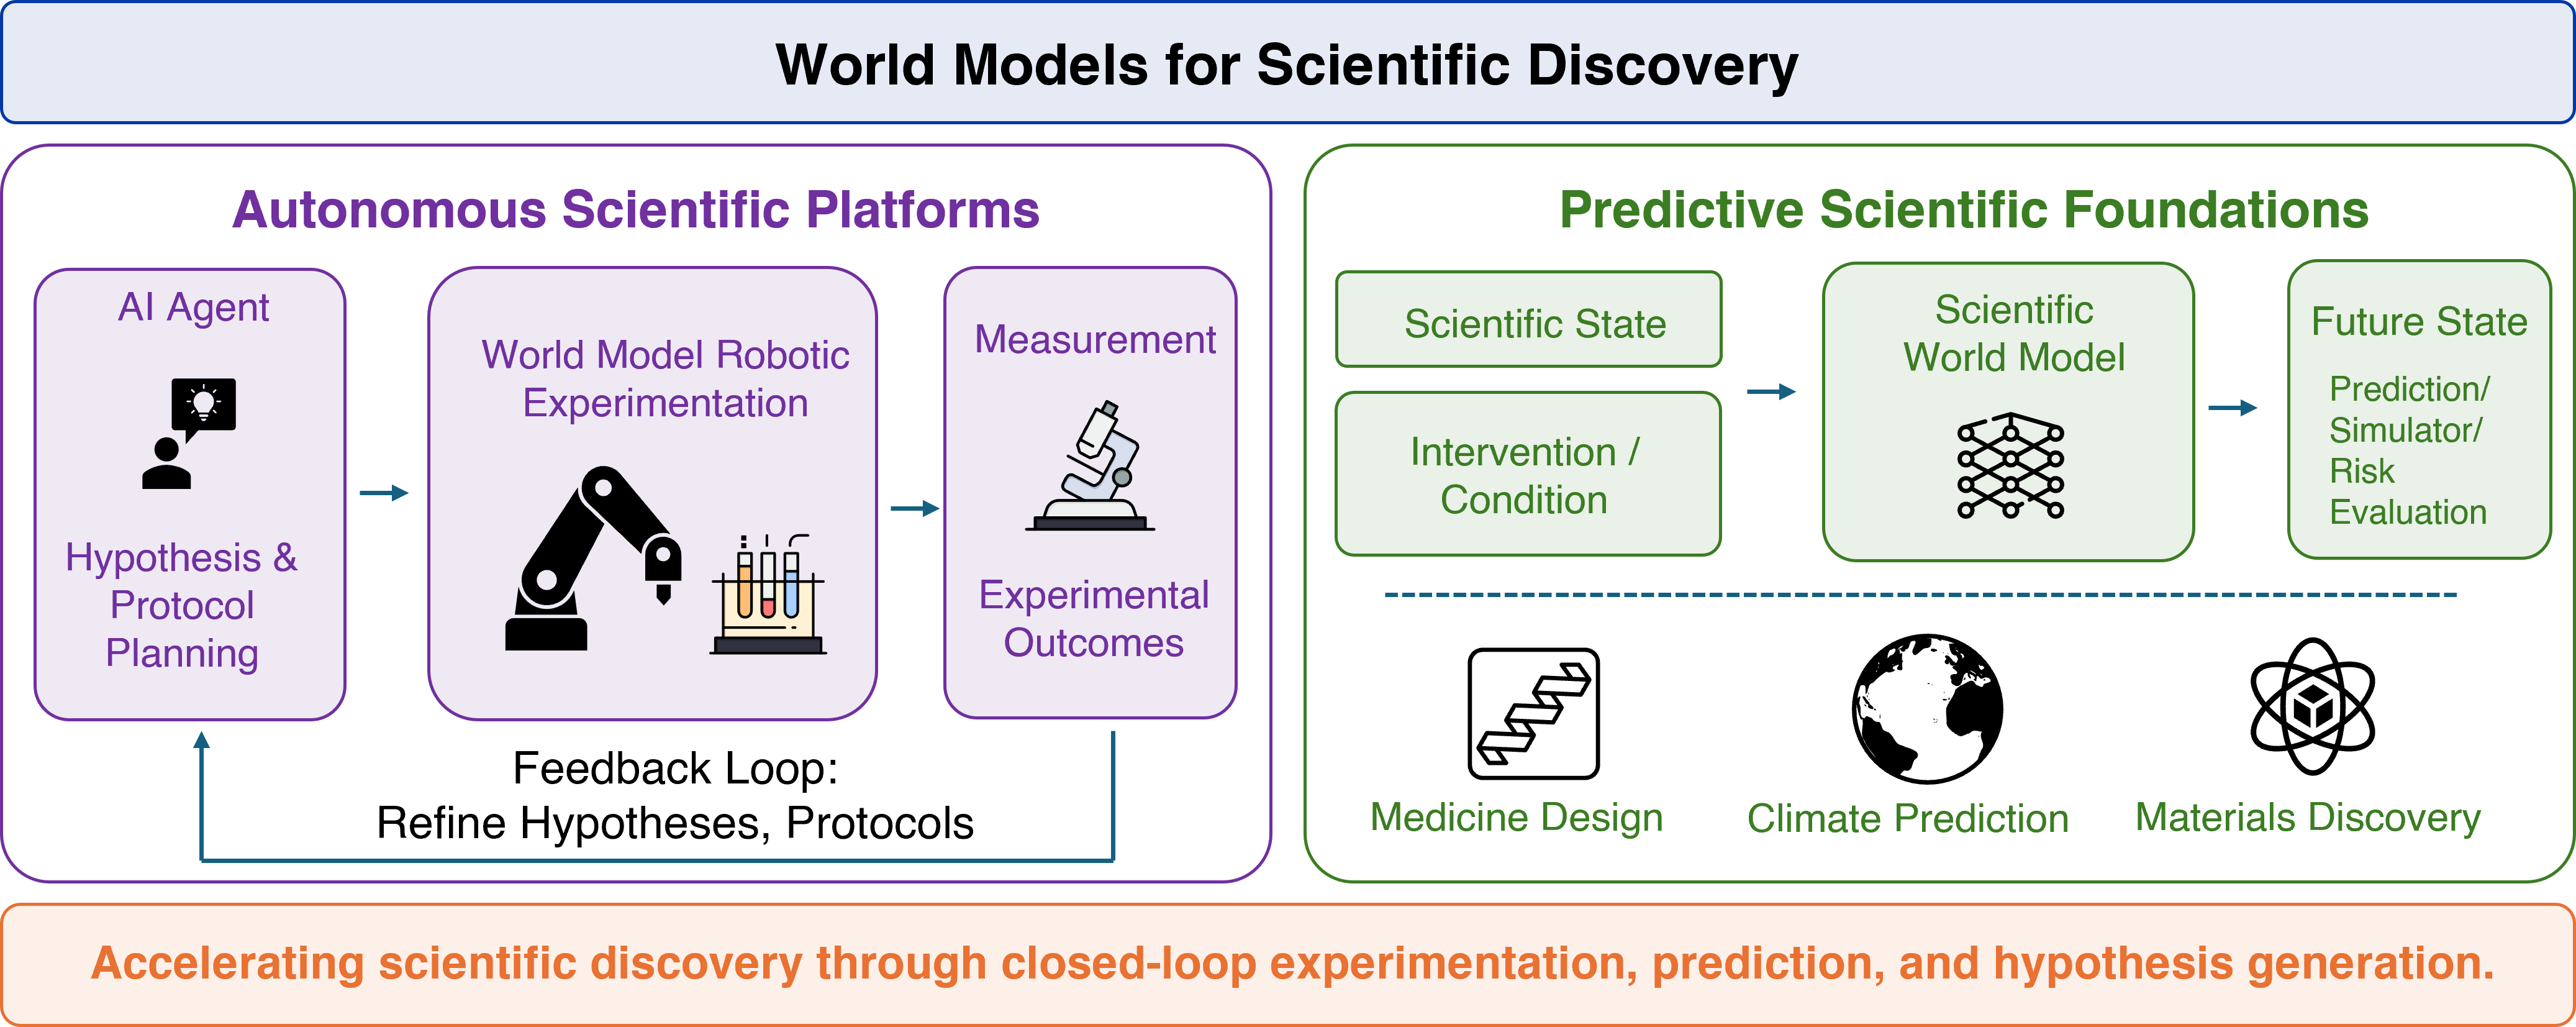
\includegraphics[width=\linewidth]{figs/science_discovery2.png}
    \caption{世界模型在科学发现中的应用。}
    \label{fig:future}
\end{figure}

世界模型已成为支撑人工智能驱动科学（AI for Science，AI4S）的基础范式，使科学发现平台能够全面进行智能化升级与优化\citep{wang2026towards}。通过提供系统性的数字框架，对客观世界的底层动力学、物理规律和运行原理建模，这些模型以两种高度互补的方式促进科学发现：赋能自主实验系统，以及充当复杂科学现象的预测基础。

首先，世界模型与人工智能智能体、机器人仪器和实验反馈结合，支持人工智能驱动的自主实验室\citep{szymanski2023autonomous,wei2025ai,wu2025ai}。它们覆盖复杂机器人操作、仪器状态动态变化等关键模态，通过协同闭环机制，与具备认知能力的大语言模型协作。真实平台部署产生的海量实验数据持续回流，用于迭代训练、改进世界模型。这形成应用驱动的双向范式：物理执行提高模型准确性，模型模拟则支持实际执行。在湿实验室中，这种整合显著提高具身系统的运行效率，使执行前的\textit{计算机内}预测推演能够预判流程与安全风险，从而减少危险，使工作流程更平顺\citep{lewis2026acht}。

其次，世界模型通过学习科学状态在不同条件或干预下如何演化，充当预测基础。它们将具身人工智能的“状态＋行动$\rightarrow$下一状态”概念扩展至科学领域，目标变为建模“科学状态＋干预／条件$\rightarrow$未来状态／响应”。科学基础模型与发现平台越来越多地支持这一角色，例如Intern-S1\citep{bai2025intern}、Intern-S1-Pro\citep{zou2026intern}和Intern-Discovery，提供推理、多模态理解、工具使用及工作流程基础设施。同时，各学科也在涌现领域专用预测世界模型。在天气与气候领域，GraphCast\citep{lam2023learning}、GenCast\citep{price2025probabilistic}、FengWu\citep{chen2023fengwu}和FengWu-W2S\citep{ling2024fengwu}等模型，将地球系统视为高维动力状态，学习其未来演化。医学与生命科学也有类似进展：Medical World Model\citep{yang2025medical}模拟以治疗为条件的肿瘤演化，Delphi-2M\citep{shmatko2025learning}则建模长期疾病进展。

最终，世界模型通过刻画超出现有人类认知边界的自然规律，推动前沿科学发现。通过符合物理规律的前向推演和反事实分析，它们识别潜在研究路径，启发新假说。这种能力不仅降低真实实验成本、加快闭环迭代，还使研究者能够探索难以直接观测的复杂过程，促进AI4S生态的长期演化与突破。
